\section{Problema \label{sec:problema}}

El problema que presenta la red de transporte el\'ectrica de buses RED es uno del tipo ``Electric Vehicle Scheduling Problem'', es decir un problema de asignaci\'on de veh\'iculos con estaciones de carga el\'ectricas. Se dispone de un conjunto de viajes programados que deben ser cubiertos durante un d\'ia de operaci\'on, cada uno definido por un paradero y hora de inicio, un paradero y hora de t\'ermino, paraderos intermedios, distancia recorrida y consumo energ\'etico asociado. Estos viajes deben asignarse a una flota de buses homog\'enea irrestricta, con un costo fijo diario por activaci\'on operacional de cada bus, de manera que cada viaje sea atendido una vez y que la secuencia asignada a cada bus constituya una cadena operacional f\'isicamente factible, es decir, un bus solo puede iniciar un viaje si tiene el tiempo suficiente para trasladarse, sin pasajeros, desde el punto donde finaliz\'o su ruta anterior hasta el inicio de la nueva. A esto se suma la autonom\'ia limitada de la bater\'ia, que debe mantenerse entre un nivel de carga m\'inimo y m\'aximo, obligando al bus a recargarse en electroterminales antes de que su carga sea cr\'itica. Estos electroterminales presentan, adem\'as, una infraestructura limitada para un n\'umero m\'aximo de buses recarg\'andose simult\'aneamente.

Dado lo anterior, se tienen tres decisiones que se deben tomar en el problema. Primero, la asignaci\'on de viajes a buses, que determina qu\'e bus ejecuta cada viaje y en qu\'e orden. Segundo, los desplazamientos sin pasajeros asociados a dicha asignaci\'on, que incluyen el trayecto de salida desde un electroterminal hacia el primer viaje del turno (\emph{pullout}), el trayecto de regreso desde el \'ultimo viaje hacia un electroterminal (\emph{pullin}), y los desplazamientos entre el t\'ermino de un viaje y el inicio del siguiente cuando ambos no son geogr\'aficamente contiguos. A estos eventos se les denomina \emph{deadheading} (o \emph{deadheads}) y tienen un costo asociado por km recorrido. Por \'ultimo, las decisiones de recarga, que implican el cu\'ando, en qu\'e electroterminal y por cu\'anto tiempo debe recargarse cada bus, sujeto a la capacidad simult\'anea de cada instalaci\'on y a que el costo de la energ\'ia var\'ia seg\'un el bloque horario en que se realice la carga.

\section{Objetivos \label{sec:objetivos}}

Con el contexto del problema ya visto, el objetivo del problema es minimizar el costo total de operaci\'on, compuesto por el costo fijo asociado al n\'umero de buses utilizados diariamente, el costo variable de los desplazamientos sin pasajeros, el costo asociado a los tiempos de espera de los buses, el costo energ\'etico de las recargas y el costo fijo asociado a cada evento de carga, sujeto a que todos los viajes programados sean cubiertos, a la factibilidad temporal y energ\'etica de la secuencia de actividades de cada bus, y a la capacidad de carga simult\'anea de los electroterminales.

\section{Entregable \label{sec:entregable}}

El entregable del proyecto es un plan operacional diario para un d\'ia laboral representativo de la red, compuesto por los siguientes elementos concretos:

\begin{itemize}
\item N\'umero m\'inimo de buses necesarios para cubrir la totalidad de las expediciones programadas.
\item Jornada operacional completa de cada bus en un archivo CSV, es decir, la secuencia ordenada de viajes que le son asignados junto con sus horarios de inicio y t\'ermino, el trayecto de \emph{pullout} desde el electroterminal de salida, los eventuales desplazamientos de \emph{deadheading} entre viajes no contiguos, y el trayecto de \emph{pullin} de regreso a un electroterminal.
\item Itinerario de recarga para cada bus en un archivo CSV, especificando en qu\'e electroterminal, en qu\'e bloque horario y por cu\'anta energ\'ia se recarga, de manera que se respeten el nivel m\'inimo de bater\'ia, la capacidad de los electroterminales y el resto de las restricciones de recarga.
\item Desglose del costo total de la soluci\'on en sus componentes (costo fijo de flota, costo de desplazamientos vac\'ios, costo de tiempos de espera, costo energ\'etico y costo fijo por evento de carga).
\end{itemize}

\section{An\'alisis de Datos \label{sec:analisisdatos}}

\subsection{Datos Disponibles \label{sec:datosdisponibles}}

Los datos utilizados provienen de tres fuentes: un archivo GTFS de RED (vigente julio-diciembre 2026) con las rutas, viajes programados, horarios, paraderos y trazados geom\'etricos de la red; un GeoPackage de OpenStreetMap con la geometr\'ia y atributos de todas las calles de Chile (nombre, tipo de v\'ia, sentido, etc.), usado para calcular distancias sin pasajeros; y un conjunto de archivos CSV con par\'ametros espec\'ificos del proyecto (ubicaci\'on y capacidad de los cinco electroterminales, potencia de los cargadores, precios de electricidad por bloque horario, caracter\'isticas t\'ecnicas del bus el\'ectrico y costos de operaci\'on). El Anexo 2 detalla cada archivo, su contenido y el uso que se le dar\'a en el proyecto.

\subsection{Filtros y Limpieza \label{sec:filtroslimpieza}}

Del archivo GTFS se conservaron \'unicamente las rutas operadas por RED, excluyendo Metro (L1 a L6), Metrotren (MTN y MTR) y una ruta de un operador externo al aeropuerto (BA), junto con sus columnas exclusivas. El feed distingue tres tipos de d\'ia (laboral, s\'abado y domingo); se filtr\'o el laboral como caso base por ser el de mayor exigencia operacional, con la mayor cantidad de rutas activas (417) y de expediciones (64.502), como muestra la Figura \ref{fig:tipodia}.

\begin{figure}[htb]
	\begin{center}
	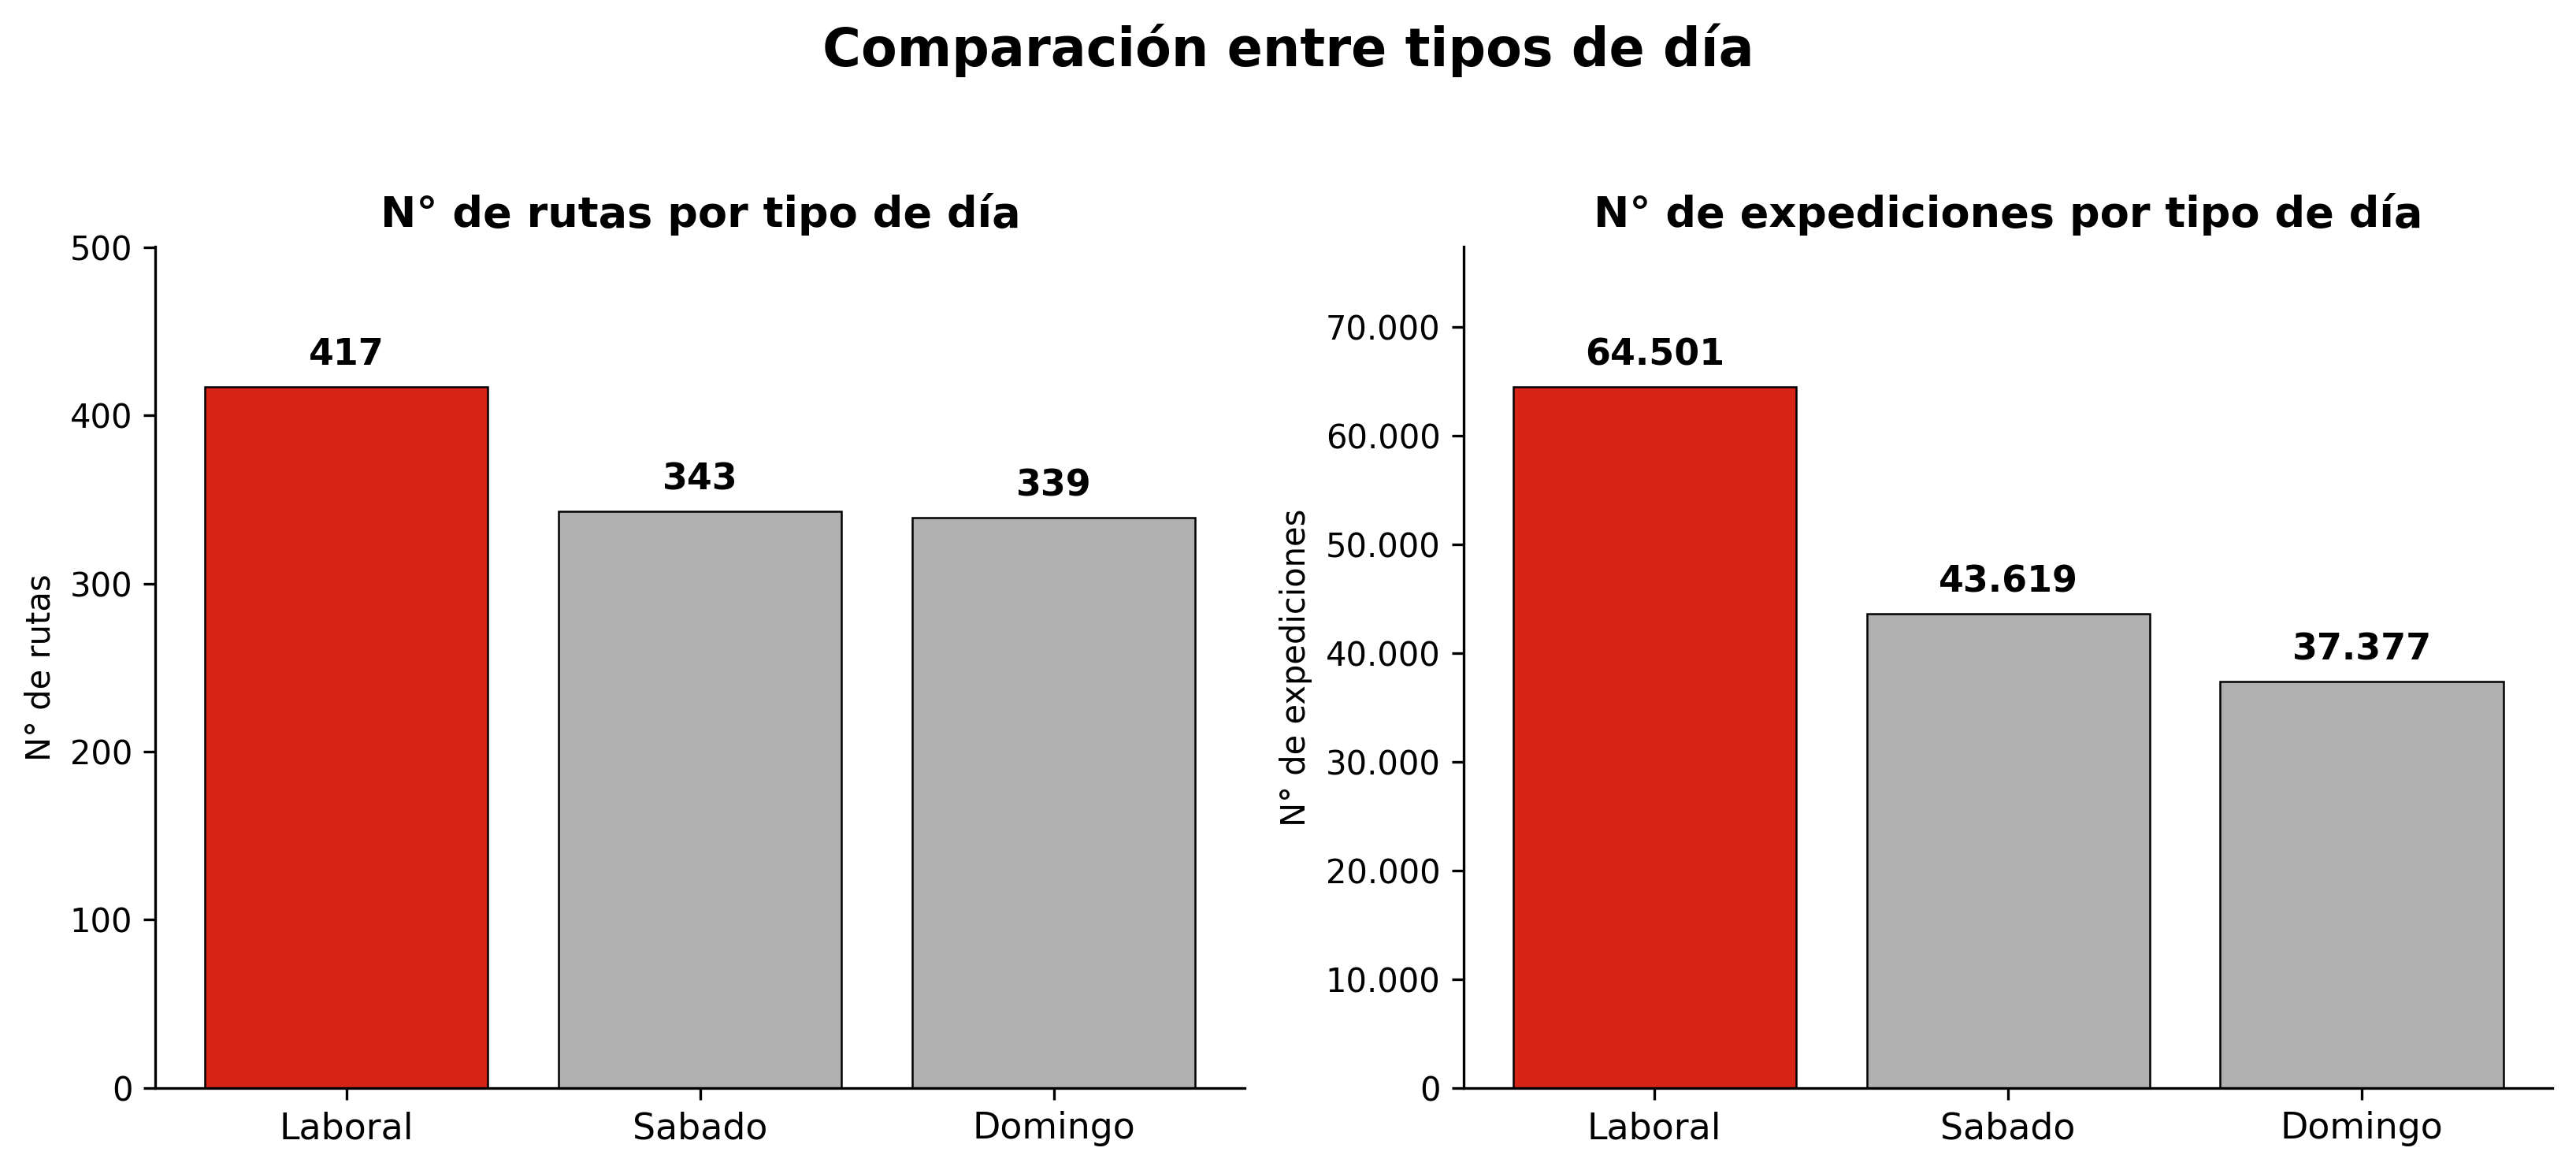
\includegraphics[width=0.65\textwidth]{./figures/grafico_tipo_dia.png}
	\caption[Comparaci\'on entre tipos de d\'ia]{Comparaci\'on entre tipos de d\'ia (n\'umero de rutas y expediciones)}
	\label{fig:tipodia}
	\end{center}
\end{figure}

Una vez filtradas las rutas de RED en d\'ias laborales, la Figura \ref{fig:mapared} muestra el mapa de las rutas que recorrer\'an los buses y la ubicaci\'on de los electroterminales donde deber\'an recargar sus bater\'ias.

\begin{figure}[htb]
	\begin{center}
	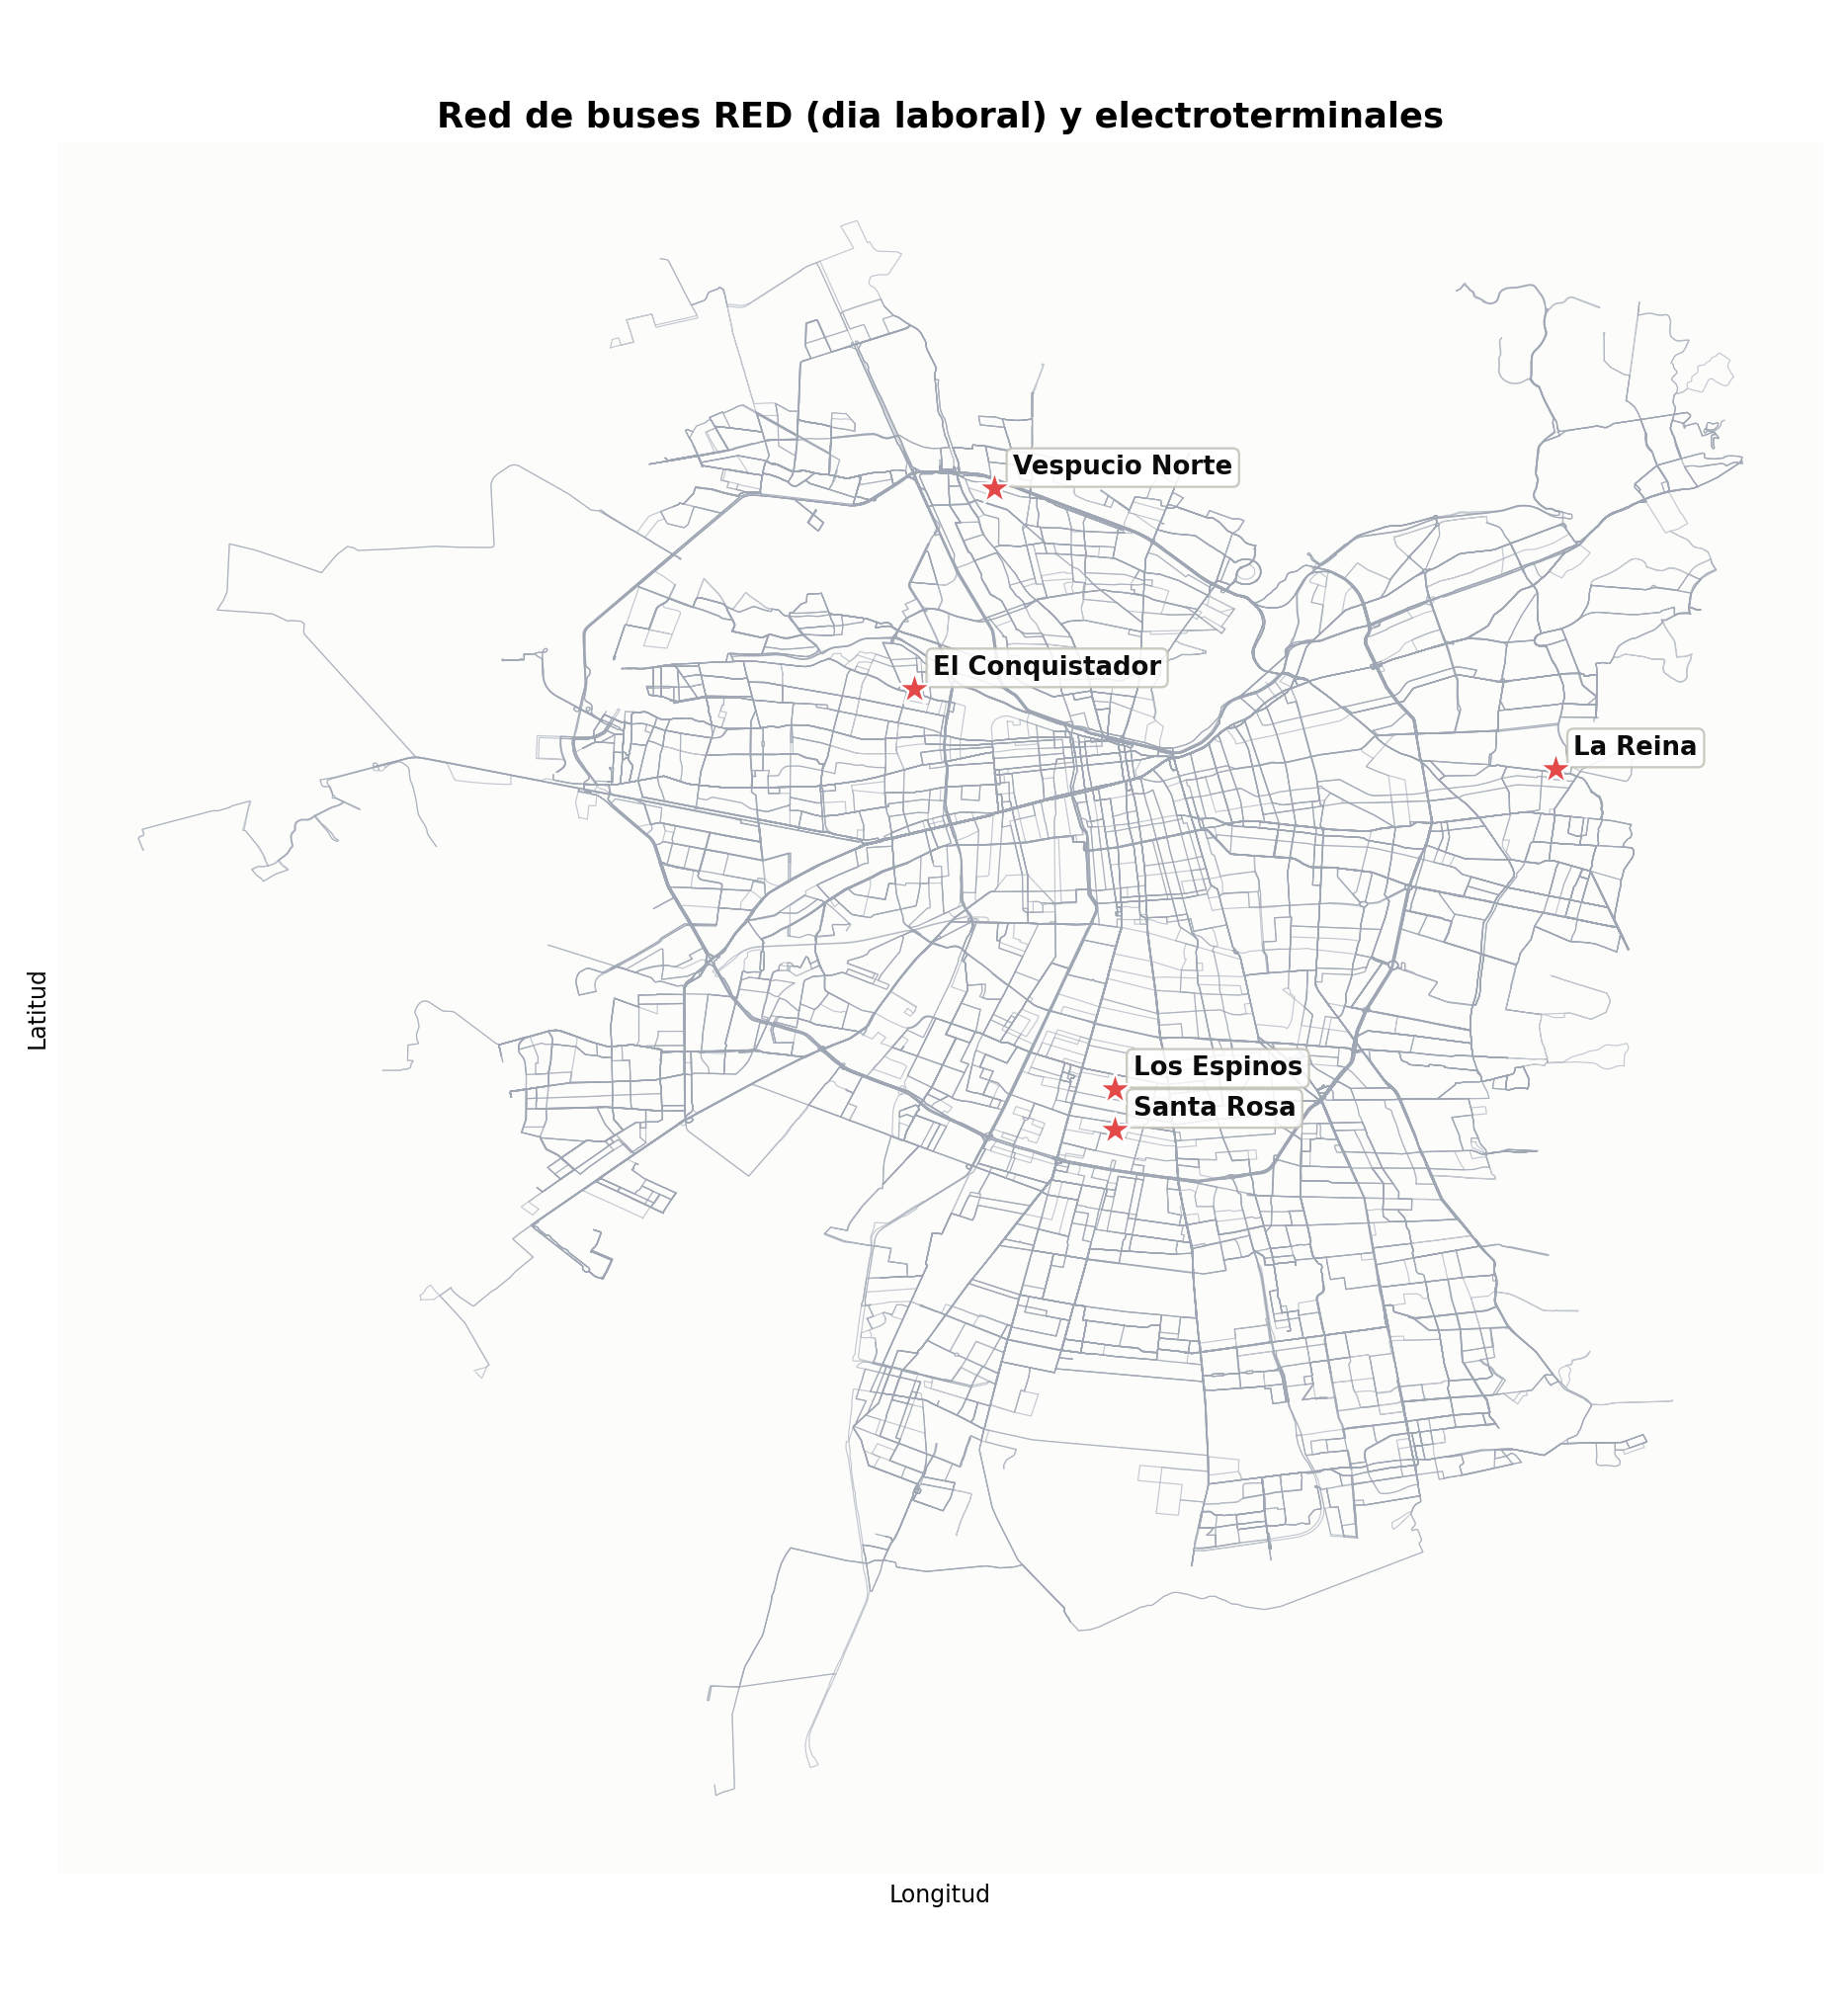
\includegraphics[width=0.5\textwidth]{./figures/mapa_rutas_electroterminales.png}
	\caption[Red de buses RED y electroterminales]{Red de buses RED (d\'ia laboral) y electroterminales}
	\label{fig:mapared}
	\end{center}
\end{figure}

El feed GTFS filtrado a RED y al d\'ia laboral contiene 417 rutas, 839 trazados geom\'etricos, 12.132 paraderos y 6.620 viajes. Al expandir estos viajes por las frecuencias definidas en el archivo \texttt{frequencies}, se obtienen 64.502 expediciones reales que deben ser cubiertas durante el d\'ia. La Tabla \ref{tab:cifrasclave} resume estas cifras.

\begin{table}[htb]
\begin{center}
\small
\caption[Cifras clave de la operaci\'on programada]{Cifras clave de la operaci\'on programada (d\'ia laboral)}
\label{tab:cifrasclave}
\begin{tabular}{@{}l r@{}}\toprule
\textbf{Indicador} & \textbf{Cantidad} \\ \midrule
Rutas & 417 \\
Trazados geom\'etricos & 839 \\
Paraderos & 12.132 \\
Viajes & 6.620 \\
Expediciones & 64.502 \\
\bottomrule
\end{tabular}
\end{center}
\end{table}

La distribuci\'on horaria de estas expediciones no es constante a lo largo del d\'ia. La Figura \ref{fig:busesporhora} muestra la cantidad de buses circulando al mismo tiempo hora a hora, donde se observan dos claros picos de demanda. El primero a las 8:00 con 6.601 buses circulando, correspondiente a entradas a oficinas y establecimientos educacionales. El segundo ocurre a las 18:00 con 6.523 buses, correspondiente al retorno de las personas a sus hogares.

\begin{figure}[htb]
	\begin{center}
	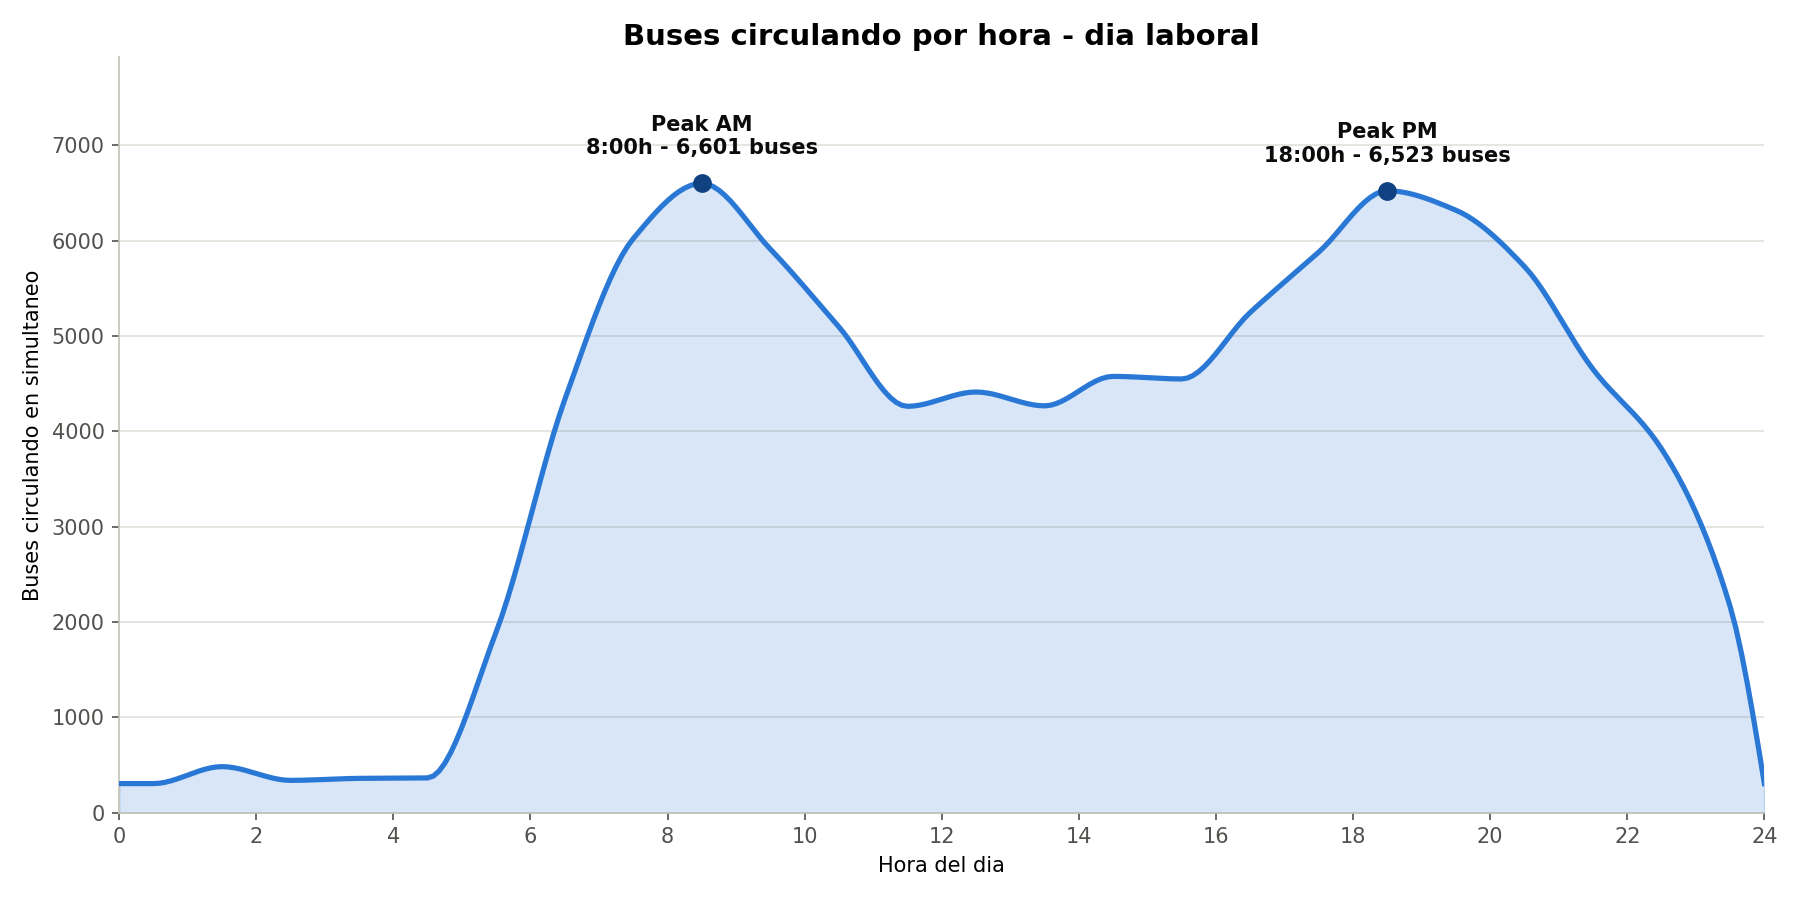
\includegraphics[width=0.65\textwidth]{./figures/buses_por_hora_curva.png}
	\caption[Buses circulando por hora]{Buses circulando por hora (d\'ia laboral)}
	\label{fig:busesporhora}
	\end{center}
\end{figure}

Esto afecta directamente a la planificaci\'on. Por una parte, la cantidad de buses necesarios para cubrir la demanda supera ampliamente la capacidad de carga simult\'anea de los electroterminales (700 espacios), por lo que las recargas deben distribuirse a lo largo del d\'ia. Por otra parte, los bloques tarifarios (Figura \ref{fig:tarifas}) tienen precios m\'as elevados justamente en las horas de mayor demanda, por lo tanto se genera una complejidad entre cubrir la demanda y minimizar el costo energ\'etico de las recargas.

\subsection{Flota e Infraestructura de Carga \label{sec:flotainfraestructura}}

La flota considerada en este proyecto es de tama\~no irrestricto y est\'a compuesta por un \'unico modelo de bus el\'ectrico, el BYD K9. La Tabla \ref{tab:especificaciones} presenta las caracter\'isticas t\'ecnicas de este veh\'iculo, las cuales definen las restricciones de autonom\'ia y recarga que deben considerarse en la planificaci\'on.

\begin{table}[htb]
\begin{center}
\small
\caption[Especificaciones t\'ecnicas bus el\'ectrico BYD K9]{Especificaciones t\'ecnicas bus el\'ectrico BYD K9}
\label{tab:especificaciones}
\begin{tabular}{@{}l r@{}}\toprule
\textbf{Par\'ametro} & \textbf{Valor} \\ \midrule
Capacidad de la bater\'ia & 350 kWh \\
Autonom\'ia m\'axima & 250 km \\
Potencia de carga & 180 kW \\
Estado de carga m\'inimo & 10\% \\
Estado de carga m\'aximo & 100\% \\
Tiempo de carga completa & 105 min \\
\bottomrule
\end{tabular}
\end{center}
\end{table}

Con una bater\'ia utilizable de 315 kWh (90\%) y un consumo de 1,4 kWh/km, la autonom\'ia real del bus es de 225 km, por lo que en jornadas extensas los buses deber\'an recargarse en electroterminales para continuar operando. La infraestructura de carga la componen 5 electroterminales distribuidos por Santiago, con una capacidad total de 700 espacios simult\'aneos.

\begin{table}[htb]
\begin{center}
\small
\caption[Capacidad de buses por electroterminal]{Capacidad de buses por electroterminal}
\label{tab:capacidadterminal}
\begin{tabular}{@{}l r@{}}\toprule
\textbf{Electroterminal} & \textbf{Capacidad} \\ \midrule
Vespucio Norte & 150 \\
El Conquistador & 180 \\
Los Espinos & 120 \\
La Reina & 100 \\
Santa Rosa & 150 \\
\midrule
Total & 700 \\
\bottomrule
\end{tabular}
\end{center}
\end{table}

Los Espinos y Santa Rosa est\'an muy cerca entre s\'i (Figura \ref{fig:mapared}), por lo que podr\'ia ser beneficioso considerarlos como un solo terminal con capacidad de 270; esta alternativa se evaluar\'a durante la ejecuci\'on del modelo.

\subsection{Costos y Tarifas \label{sec:costostarifas}}

Como vimos anteriormente, la funci\'on objetivo del problema busca minimizar el costo total de operaci\'on, el cual se compone de cuatro componentes principales. La Tabla \ref{tab:costos} resume los valores de cada costo.

\begin{table}[htb]
\begin{center}
\small
\caption[Costos operacionales del sistema]{Costos operacionales del sistema}
\label{tab:costos}
\begin{tabular}{@{}l r@{}}\toprule
\textbf{Tipo de costo} & \textbf{Precio} \\ \midrule
Costo fijo por uso de bus & 250 USD \\
Costo por minuto de espera & 0,03 USD/min \\
Costo por km recorrido & 0,5 USD/km \\
Costo fijo por recarga & 5 USD \\
\bottomrule
\end{tabular}
\end{center}
\end{table}

El costo fijo por bus incentiva a usar la menor cantidad de buses posible, dado que la flota es irrestricta. El costo por km recorrido incluye tanto los desplazamientos con pasajeros como \emph{deadheading}, \emph{pullin} y \emph{pullout}. El costo de espera penaliza los tiempos muertos entre viajes de un mismo bus, y el costo fijo por recarga se aplica cada vez que un bus entra a un electroterminal.

Adem\'as, el costo de la energ\'ia depende del periodo horario de consumo, y va desde 0,10 USD/kWh en el bloque valle (0-8h) hasta 0,22 USD/kWh en los bloques peak (14-17h y 19-22h), como muestra la Figura \ref{fig:tarifas}. El modelo debe encontrar un equilibrio entre cargar en bloques de menor costo y garantizar que todos los buses tengan energ\'ia suficiente para sus viajes asignados.

\begin{figure}[htb]
	\begin{center}
	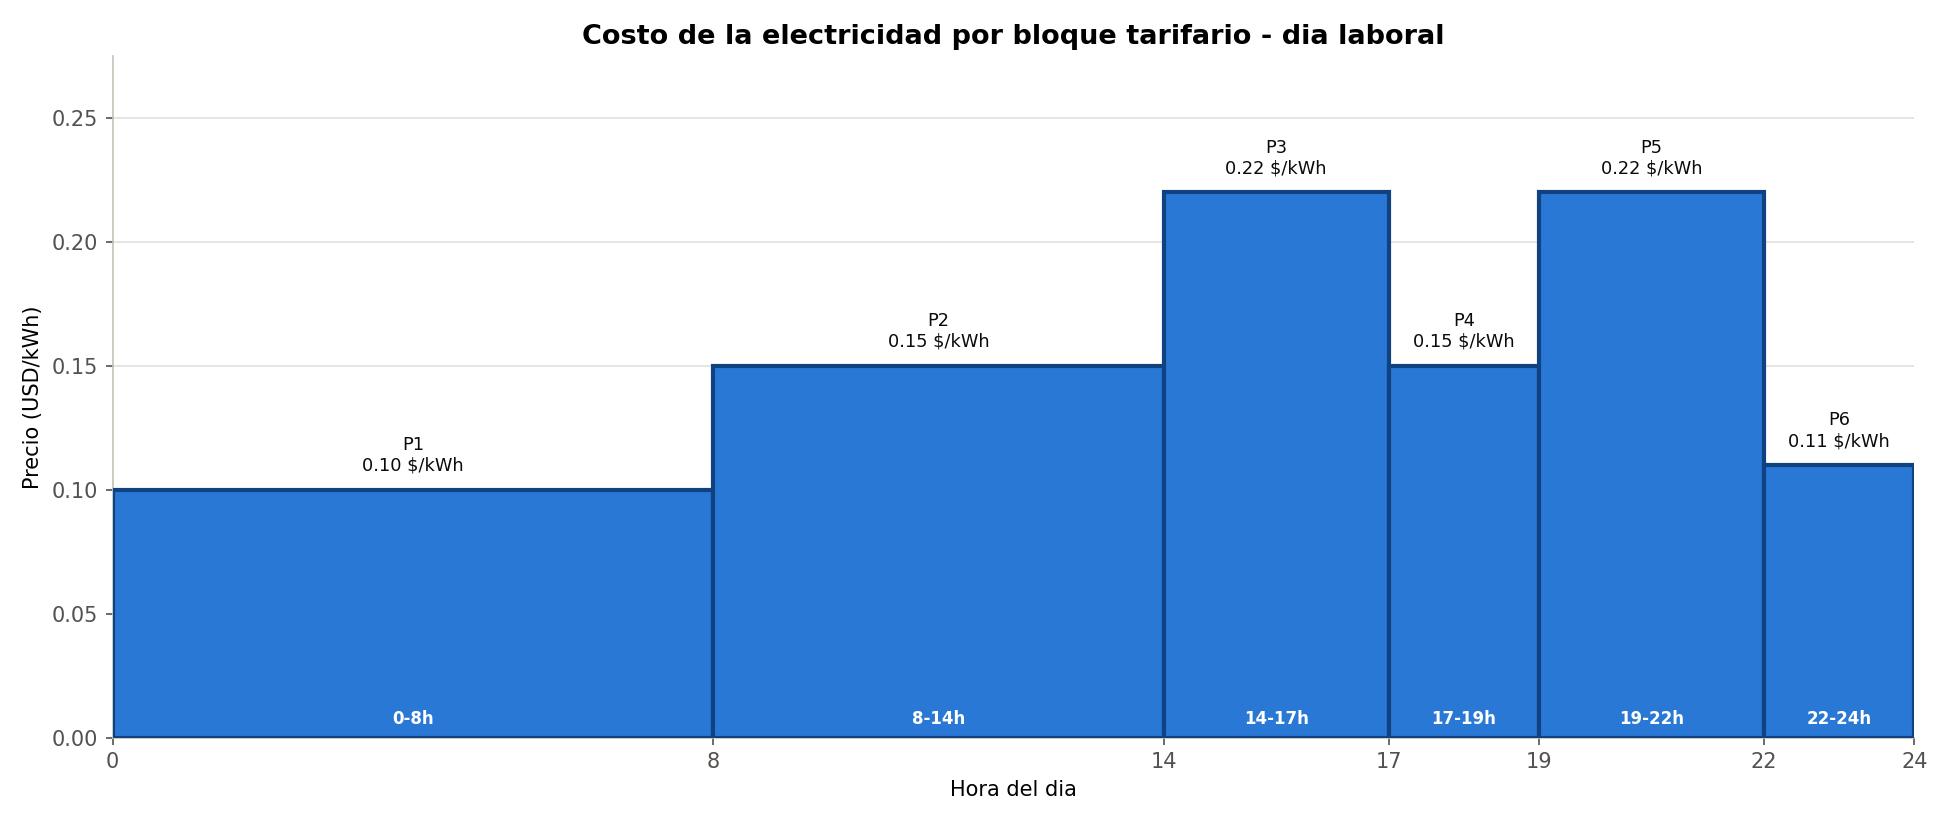
\includegraphics[width=0.6\textwidth]{./figures/costo_energia_por_periodo.png}
	\caption[Costo de la electricidad por bloque tarifario]{Costo de la electricidad por bloque tarifario (d\'ia laboral)}
	\label{fig:tarifas}
	\end{center}
\end{figure}

\subsection{Datos No Disponibles \label{sec:datosnodisponibles}}

Si bien los datos cubren la mayor parte de la informaci\'on necesaria para modelar el problema, algunos elementos no est\'an disponibles y deben aproximarse o calcularse. La duraci\'on de los viajes y las distancias de \emph{deadheading} se calculan con una velocidad promedio constante, sin considerar congesti\'on horaria ni topograf\'ia (por ejemplo, mayor pendiente en comunas precordilleranas). No se cuenta con informaci\'on de turnos de conductores, ya que el modelo planifica solo la operaci\'on del veh\'iculo, suponiendo siempre un conductor disponible. Tampoco se dispone de la demanda real de pasajeros, por lo que se usa la oferta programada (expediciones) como demanda a cumplir. Adem\'as, no existe un identificador de bloque de veh\'iculo (\texttt{block\_id}) t\'ipico de GTFS, por lo que la asignaci\'on de viajes debe construirse desde cero; tampoco hay distancias y tiempos de \emph{deadheading}, \emph{pullin} y \emph{pullout} (se calcular\'an desde la red vial de OpenStreetMap), ni energ\'ia consumida por viaje (se deriva multiplicando la distancia del trazado por el consumo de 1,4 kWh/km).

\section{KPIs \label{sec:kpis}}

Para evaluar la calidad de las soluciones generadas por el modelo, se definen cuatro indicadores de desempe\~no relevantes, alineados con el objetivo del problema.

\begin{itemize}
\item \textbf{N\'umero total de buses usados}: Indica la cantidad de buses despachados durante la jornada. Es un indicador importante para el objetivo del problema, porque la flota es de tama\~no irrestricto y cada bus utilizado incurre en un costo fijo de 250 USD.
\item \textbf{Costo energ\'etico promedio}: Se calcula como el costo total de energ\'ia dividido por los kWh totales cargados durante la jornada. Con este indicador se puede evaluar si las recargas se est\'an realizando en bloques tarifarios m\'as econ\'omicos o m\'as caros.
\item \textbf{Proporci\'on de deadheading/pullin/pullout}: Se calcula como la suma de kil\'ometros recorridos sin pasajeros (\emph{deadheading} entre viajes, \emph{pullout} desde electroterminal y \emph{pullin} de regreso) dividida por los kil\'ometros totales recorridos por la flota. Este indicador mide la eficiencia geogr\'afica de la asignaci\'on de viajes. El modelo debe buscar encadenar viajes geogr\'aficamente cercanos para minimizar este indicador.
\item \textbf{Utilizaci\'on por bus}: Se define como la raz\'on entre las horas con pasajeros y las horas totales del turno de cada bus. Con esto se eval\'ua cu\'anto del tiempo productivo de cada bus efectivamente se destina a servicio. Una utilizaci\'on alta indica que los buses pasan la mayor parte de su jornada transportando pasajeros, con tiempos de espera y recarga bien coordinados. Por el contrario, una utilizaci\'on muy baja indica problemas con la secuencia de viajes asignados.
\end{itemize}
